\tikzset{every picture/.style={line width=0.75pt}} %set default line width to 0.75pt        
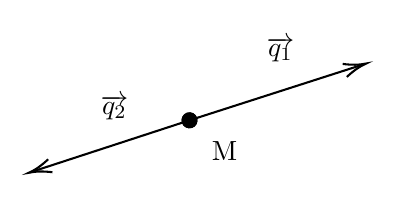
\begin{tikzpicture}[x=0.75pt,y=0.75pt,yscale=-1,xscale=1]
%uncomment if require: \path (0,92); %set diagram left start at 0, and has height of 92
%Straight Lines [id:da19898209267326417] 
\draw    (326.16,55.24) -- (409.47,28.47) ;
\draw [shift={(411.37,27.86)}, rotate = 522.19] [color={rgb, 255:red, 0; green, 0; blue, 0 }  ][line width=0.75]    (10.93,-3.29) .. controls (6.95,-1.4) and (3.31,-0.3) .. (0,0) .. controls (3.31,0.3) and (6.95,1.4) .. (10.93,3.29)   ;
\draw [shift={(326.16,55.24)}, rotate = 342.19] [color={rgb, 255:red, 0; green, 0; blue, 0 }  ][fill={rgb, 255:red, 0; green, 0; blue, 0 }  ][line width=0.75]      (0, 0) circle [x radius= 3.35, y radius= 3.35]   ;
%Straight Lines [id:da5450424757830004] 
\draw    (326.16,55.24) -- (250.59,79.91) ;
\draw [shift={(248.69,80.53)}, rotate = 341.91999999999996] [color={rgb, 255:red, 0; green, 0; blue, 0 }  ][line width=0.75]    (10.93,-3.29) .. controls (6.95,-1.4) and (3.31,-0.3) .. (0,0) .. controls (3.31,0.3) and (6.95,1.4) .. (10.93,3.29)   ;
\draw [shift={(326.16,55.24)}, rotate = 161.92] [color={rgb, 255:red, 0; green, 0; blue, 0 }  ][fill={rgb, 255:red, 0; green, 0; blue, 0 }  ][line width=0.75]      (0, 0) circle [x radius= 3.35, y radius= 3.35]   ;
% Text Node
\draw (343,70) node   [align=left] {M};
% Text Node
\draw (370,21) node    {$\overrightarrow{q_{1}}$};
% Text Node
\draw (290,49) node    {$\overrightarrow{q_{2}}$};
\end{tikzpicture}